% ---------
% --------
%!TEX TS-program = pdflatex
%!TEX encoding = UTF-8 Unicode
%!TEX spellcheck = English (Aspell)

\documentclass[11pt]{article}
\usepackage{lucy,handout,graphicx}
\usepackage{fourier-orns}
\usepackage{mathtools}
\usepackage[normalem]{ulem} % either use this (simple) or
\usepackage{tikz}
\usetikzlibrary{graphs}

\allowdisplaybreaks


\begin{document}

\noindent Name \underline{\hspace{12cm}}\\

\begin{center}
\Large\textbf{CSCI 332, Fall 2026}\\
\LARGE\textbf{Exam 1 Practice 2}
\end{center}

\noindent This exam consists of the following sections:
\begin{enumerate}
    \item Stable Matching (25 points)
    \item Algorithm Analysis (25 points)
    \item Recursion (25 points)
    \item Backtracking and 1D Dynamic Programming (25 points)
\end{enumerate}

You may use a double sided 3x5 handwritten notecard of notes during the test but no other resources.

Good luck!

\newpage

\begin{center}
\LARGE\textbf{Section 1 (Stable Matching)\\}%
\end{center}


\begin{enumerate}

\item Given the matching
$\{(h_4, s_1), (h_1, s_3), (h_3, s_4), (h_2, s_2), (h_5, s_5)\}$ and the
preference lists below,
select the unstable pairs for this matching from the list below by circling them.

\begin{table}[h]
\centering
\begin{tabular}{c|ccccc}
\textbf{Hospital} & \textbf{1st choice} & \textbf{2nd choice} & \textbf{3rd choice} & \textbf{4th choice} & \textbf{5th choice} \\
\hline
$h_1$ & $s_1$ & $s_2$ & $s_5$ & $s_3$ & $s_4$ \\
$h_2$ & $s_4$ & $s_5$ & $s_1$ & $s_3$ & $s_2$ \\
$h_3$ & $s_1$ & $s_5$ & $s_2$ & $s_3$ & $s_4$ \\
$h_4$ & $s_3$ & $s_2$ & $s_4$ & $s_1$ & $s_5$ \\
$h_5$ & $s_1$ & $s_4$ & $s_2$ & $s_5$ & $s_3$ \\
\hline
\textbf{Student} & \textbf{1st choice} & \textbf{2nd choice} & \textbf{3rd choice} & \textbf{4th choice} & \textbf{5th choice} \\
\hline
$s_1$ & $h_2$ & $h_4$ & $h_3$ & $h_1$ & $h_5$ \\
$s_2$ & $h_4$ & $h_2$ & $h_5$ & $h_1$ & $h_3$ \\
$s_3$ & $h_4$ & $h_3$ & $h_2$ & $h_1$ & $h_5$ \\
$s_4$ & $h_3$ & $h_4$ & $h_5$ & $h_1$ & $h_2$ \\
$s_5$ & $h_4$ & $h_1$ & $h_5$ & $h_3$ & $h_2$ \\
\end{tabular}
\end{table}

\begin{enumerate}[(a)]
    \item $(h_5, s_4)$
    \item $(h_3, s_3)$
    \item $(h_3, s_4)$
    \item $(h_4, s_3)$
    \item $(h_1, s_4)$
\end{enumerate}
\newpage

Your friend proposes the following, simple algorithm for stable matching:

    \begin{algo}
    Gale-Shapley-Simplified(preference lists for $n$ hospitals and $n$ students)\+\\
    Let $M$ be an empty matching\\
    While some hospital $h$ is umatched:\+ \\
        Let $s$ be the first student on $h$'s preference list that is not yet matched\\
        Add $(h,s)$ to $M$\-\\
    Return $M$\\
    \end{algo}

\item What are the best-case and worst-case $\Theta$ runtimes for this algorithm in terms of $n$? You should
give the simplest function possible.

\vspace{2in}

\item Is the algorithm correct? If yes, simply write ``yes''. If not, give an instance for which
Gale-Shapley-Simplified does not return a stable matching.

\newpage


\begin{center}
\LARGE\textbf{Section 2 (Algorithm Analysis)\\}%
\end{center}

\item 
Suppose you have algorithms with the following runtimes.
(Assume these are exact running times as a function of the input size $n$, not
asymptotic running times.) How much slower do these algorithms get when you
double the input size? (You can find this by dividing the runtime on $2n$ by the
runtime on $n$). You should simplify your answer as much as possible, including evaluating
logarithms when possible.

\begin{enumerate}[(a)]
    \item $3n^2$ 
\vspace{1in}
    \item $\log_2 n$
\vspace{1in}
    \item $3^{n}$
\vspace{1in}
\end{enumerate}


\item 
Order the following functions from asymptotically smallest to asymptotically
largest by labeling the smallest with a 1 and increasing from there.  If two
functions are asymptotically equal (one is $\Theta$ of the other), give them the
same number. For example, if the functions were $n$, $n^2$, and $3n + 4$, the
labels should be 1, 2, 1.

    \begin{itemize}
        \item[\underline{\hspace{0.5cm}}] $n \log n^3$
        \item[\underline{\hspace{0.5cm}}] $n \log n^2$
        \item[\underline{\hspace{0.5cm}}] $\sqrt{n}$
        \item[\underline{\hspace{0.5cm}}] $n + \log n$
        \item[\underline{\hspace{0.5cm}}] $n^{\log_3 2}$
        \item[\underline{\hspace{0.5cm}}] $100^{100!}$
        \item[\underline{\hspace{0.5cm}}] $\log_2 n$
        \item[\underline{\hspace{0.5cm}}] $2^n$
        \item[\underline{\hspace{0.5cm}}] $3^n$
    \end{itemize}

    \newpage

\item

Suppose you know that an algorithm has a worst-case runtime that is $O(n^2 \log n)$. For each of the following, decide whether it is definitely true, definitely false, or could be true or false and circle your choice. 

\begin{itemize}
    \item The algorithm's worst-case runtime is $\Omega(n^2)$. T, F, T or F
    \item The algorithm's worst-case runtime is $\Omega(n^3)$. T, F, T or F
    \item The algorithm's best-case runtime is $O(n^2)$. T, F, T or F
    \item The algorithm's worst-case runtime is $O(n^3)$. T, F, T or F
    \item The algorithm's worst-case runtime is $\Theta(n^2 \log n)$. T, F, T or F
\end{itemize}



\newpage

\begin{center}
\LARGE\textbf{Section 3 (Recursion)\\}%
\end{center}
 

\item Given the following (meaningless) divide and conquer algorithm,
what is the recurrence relation that describes its runtime? Indicate your answer by circling it.
Notice the $n$ is the number of rows and the number of columns in the square array $A$,
not the total number of elements.

    \begin{algo}
    hi(square array $A$ of with $n$ rows and $n$ columns): \+ \\
    if $n = 1$:\+\\
        return $sum(A)$\-\\
    else:\+\\
    Let $A_1, A_2, A_3, A_4$ be the upper left, upper right, lower left, and lower right of $A$\\
    $X_1$ = hi($A_1$ + $A_4$)\\
    $X_2$ = hi($A_2$ + $A_3$)\\
    $C$ = $X_1$ + $X_2$\\
    return $C$\-\\
    \end{algo}

\begin{enumerate}[A.]
    \item $T(n) = 2T(n^2/2) + \Theta(n^2)$
    \item $T(n) = T(n/2) + \Theta(n^2)$
    \item $T(n) = 2T(n/2) + \Theta(n^2)$
    \item $T(n) = 2T(n/2) + \Theta(n)$
    \item $T(n) = 2T(n-2) + \Theta(n^2)$
\end{enumerate}

\item[] The next two questions refer to the recurrence relation
\[T(n) = 3T(n/4) + \Theta(n^2).
\]
\item What is the work done at each level of the recursion tree for this recurrence? Circle your answer.
\begin{enumerate}[A.]
    \item $3^{\ell} + n^2$
    \item $3^{\ell} \left(\frac{n}{4^\ell}\right)^2$
    \item $\frac{4}{3} \ell^n$
    \item $n^2/4 + 3^\ell$
    \item $\frac{\ell \cdot n^2}{3}$
\end{enumerate}

\item How many levels does the recursion tree have? Circle your answer.

\begin{enumerate}[A.]
    \item $\log_4 n$
    \item $\log_3 n$
    \item $n$
    \item $^3\sqrt{n}$
    \item $n \log_3 4$

\end{enumerate}

The following questions refer to the problem of multiplying two n-digit
numbers.

\item Below is a divide and conquer algorithm to multiply two n-digit numbers $x$
and $y$ based on the observation that, if $a$ and $b$ are the first and second halves
of $x$ and $c$, and $d$ are the first and second halves of $y$ respectively, then

\[
x \cdot y = 10^n \cdot a \cdot c + 10^{n/2} \cdot (a \cdot d + b \cdot c) + b \cdot d.
\]

    \begin{algo}
    Split-Multiply(length $n$ integers $x$, $y$):\+\\
    \# base case\\
    if $n = 1$:\+\\
        return \underline{\hspace{1in}}\- \\
    \\
    \# recursive case\\
    else:\+\\
    Split $x$ into two halves $a$ and $b$\\
    Split $y$ into two halves $c$ and $d$\\
    $m=n/2$\\
    $e = $ Split-Multiply($a$, $c$) \\
    $f = $ Split-Multiply($b$, $d$) \\
    $g = $ Split-Multiply($b$, $c$) \\
    $h = $ Split-Multiply($a$, $d$) \\
    return $10^{2m} \cdot e + 10^{m} \cdot (g + h) + f$
    \end{algo} 

What should be returned in the base case (the blank above)? Circle your answer.
\begin{enumerate}[A.]
    \item $0$
    \item $1$
    \item $x + y$
    \item $x \cdot y$
    \item $x - y$
\end{enumerate}

\item If $x=1234$ and $y=5678$, what are the values of $a$, $b$, $c$, and $d$ when
Split-Multiply($x,y,4$) is called?
\begin{enumerate}[A.]
    \item $a=12$, $b=34$, $c=56$, $d=78$
    \item $a=1$, $b=234$, $c=5$, $d=678$
    \item $a=123$, $b=4$, $c=567$, $d=8$
    \item $a=1234$, $b=0$, $c=5678$, $d=0$
    \item $a=0$, $b=1234$, $c=0$, $d=5678$  
\end{enumerate}

\item What is the runtime of Split-Multiply as a function of $n$, the number of digits
in the input numbers $x$ and $y$?
\begin{enumerate}[A.]
    \item $\Theta(n)$
    \item $\Theta(n \log n)$
    \item $\Theta(n^2)$
    \item $\Theta(n^{\log_2 3})$
    \item $\Theta(2^n)$
\end{enumerate}
\newpage


\begin{center}
\LARGE\textbf{Section 4 (1D Dynamic Programming)\\}%
\end{center}

Having spied some snow on the mountains, you are thinking
about ski season. You will ski a ski jumping course with $n$ jumps, each evenly spaced one
meter apart. The height that each jump will launch you is stored in an array $H[1..n]$. However,
each jump will also launch you 2 meters in horizontal distance, meaning that if you take a jump,
you must skip the next jump. You can always choose to skip a jump.
You would like to accumulate the largest total height jumped by choosing a set of jumps to take. 

\begin{enumerate}
    \item Suppose the jump heights are given by the following array (indices noted above):
    \begin{center}
    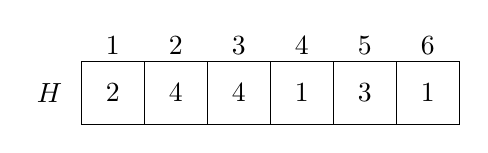
\begin{tikzpicture}[x=0.8cm,y=0.8cm]
        \node[anchor=east] at (-0.15,0) {$H$};
        \foreach \x/\i/\h in {0.5/1/2, 1.5/2/4, 2.5/3/4, 3.5/4/1, 4.5/5/3, 5.5/6/1} {
            \node at (\x,0.75) {\i};
            \node[draw, rectangle, text width=0.8cm, minimum height=0.8cm, inner sep=0pt, align=center] at (\x,0) {\h};
        }
    \end{tikzpicture}
    \end{center}

    What is the optimal set of jumps to take and what is the total height?
    \vspace{1in}

\item To solve this problem, you decide on the following English definition of the subproblems.

    \textbf{The subproblem.} Let $MaxHeight(i)$ be the maximum total height you can jump,
    assuming you only consider jumps $i$ through $n$.

    What is $MaxHeight(4)$ for the above $H$?
    \vspace{1in}

    Next, we think about the recursive relationship between subproblems.  You notice that you have two
    choices: either take the $i$th jump, or don't.
    \item 
    \textbf{The recursive definition.} 


    \begin{equation*}
        MaxHeight(i) =
        \begin{cases}
        \underline{\hspace{3in}} & if i \underline{\hspace{1in}} \\
        \underline{\hspace{3in}} & if i \underline{\hspace{1in}} \\
        \underline{\hspace{3in}} & if i \underline{\hspace{1in}} \\
        \underline{\hspace{3in}} & if i \underline{\hspace{1in}} \\
        \underline{\hspace{3in}} & if i \underline{\hspace{1in}} \\
        \end{cases}
    \end{equation*}

    \newpage

    \textbf{How to memoize?}
    We can store solutions to the subproblems in an array. What direction should we fill it (left to right or right to left)?
    \vspace{1in}

    \item 

    \textbf{Write the full algorithm.} Using the above information, finish the pseudocode
    to find the maximum amount of air you can get on the ski jumps,
    given $H[1..n]$.
    \begin{algo}
    SkiJump($H[1..n]$):\+\\
    Let array $M$ be an array of length $n$\\
    \# do we have any base cases?\\
    \\
    \\
    \\
    \\
    \\
    \# how should we fill in the rest of the array?\\
    \\
    \\
    \\
    \\
    \\
    \\
    \\
    \\
    \# what should we return to get the final answer?\\
    \\
    \\
    \\
    \hspace{5in}
    \end{algo}
\end{enumerate}
\end{enumerate}
\end{document}
